\documentclass[tikz,border=8pt]{standalone}

\begin{document}
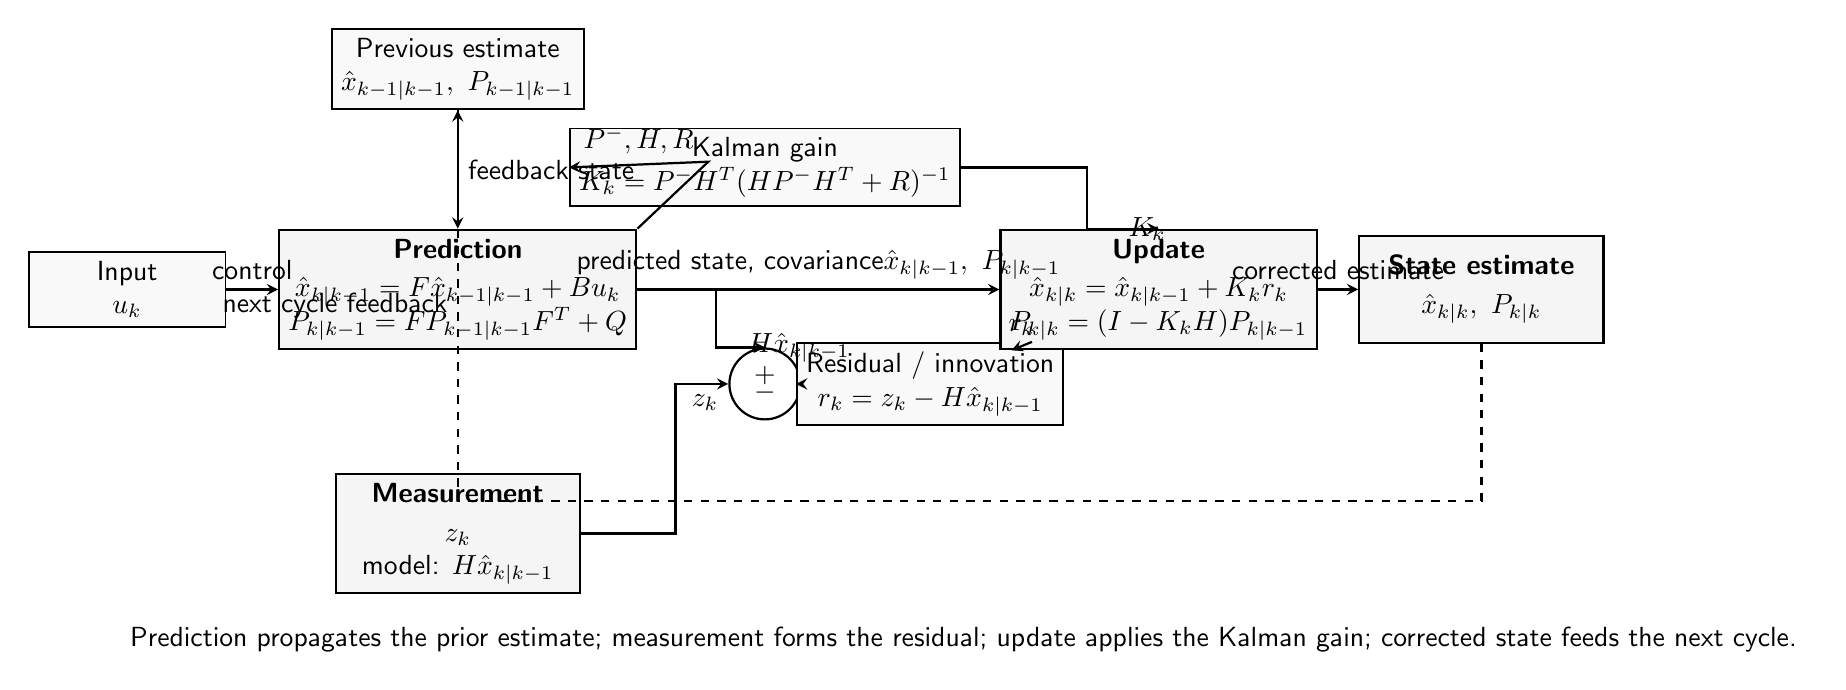
\begin{tikzpicture}[
  font=\sffamily,
  >=stealth,
  block/.style={
    draw,
    rectangle,
    align=center,
    minimum width=3.1cm,
    minimum height=1.35cm,
    line width=0.8pt,
    fill=gray!8
  },
  smallblock/.style={
    draw,
    rectangle,
    align=center,
    minimum width=2.5cm,
    minimum height=0.9cm,
    line width=0.7pt,
    fill=gray!5
  },
  sum/.style={
    draw,
    circle,
    align=center,
    minimum size=0.9cm,
    line width=0.8pt
  },
  arrow/.style={->, line width=0.8pt},
  feedback/.style={->, line width=0.8pt, dashed}
]

\node[smallblock] (input) at (-4.2, 2.2) {Input\\$u_k$};

\node[block] (prediction) at (0, 2.2) {
  \textbf{Prediction}\\[2pt]
  $\hat{x}_{k|k-1}=F\hat{x}_{k-1|k-1}+Bu_k$\\
  $P_{k|k-1}=FP_{k-1|k-1}F^T+Q$
};

\node[smallblock] (gain) at (3.9, 3.75) {
  Kalman gain\\
  $K_k=P^-H^T(HP^-H^T+R)^{-1}$
};

\node[sum] (residual) at (3.9, 1.0) {$+$\\[-6pt]$-$};

\node[block] (measurement) at (0, -0.9) {
  \textbf{Measurement}\\[2pt]
  $z_k$\\
  model: $H\hat{x}_{k|k-1}$
};

\node[smallblock] (innovation) at (6.0, 1.0) {
  Residual / innovation\\
  $r_k=z_k-H\hat{x}_{k|k-1}$
};

\node[block] (update) at (8.9, 2.2) {
  \textbf{Update}\\[2pt]
  $\hat{x}_{k|k}=\hat{x}_{k|k-1}+K_kr_k$\\
  $P_{k|k}=(I-K_kH)P_{k|k-1}$
};

\node[block] (estimate) at (13.0, 2.2) {
  \textbf{State estimate}\\[2pt]
  $\hat{x}_{k|k},\ P_{k|k}$
};

\node[smallblock] (prev) at (0, 5.0) {
  Previous estimate\\
  $\hat{x}_{k-1|k-1},\ P_{k-1|k-1}$
};

\draw[arrow] (input) -- node[above] {control} (prediction);
\draw[arrow] (prev) -- node[right] {feedback state} (prediction);

\draw[arrow] (prediction) -- node[above] {predicted state, covariance\\$\hat{x}_{k|k-1},\ P_{k|k-1}$} (update);

\draw[arrow] (prediction.east) -- ++(1.0,0) |- node[pos=0.72, right] {$H\hat{x}_{k|k-1}$} (residual.north);
\draw[arrow] (measurement.east) -- ++(1.2,0) |- node[pos=0.78, below] {$z_k$} (residual.west);

\draw[arrow] (residual) -- (innovation);
\draw[arrow] (innovation) -- node[above] {$r_k$} (update);

\draw[arrow] (prediction.north east) -- ++(0.9,0.85) -- node[above] {$P^-,H,R$} (gain.west);
\draw[arrow] (gain.east) -- ++(1.6,0) |- node[pos=0.72, right] {$K_k$} (update.north);

\draw[arrow] (update) -- node[above] {corrected estimate} (estimate);

\draw[feedback] (estimate.south) -- ++(0,-2.0) -- ++(-13.0,0) -- node[left] {next cycle feedback} (prev.south);

\node[align=center] at (6.5, -2.25) {
  Prediction propagates the prior estimate; measurement forms the residual; update applies the Kalman gain; corrected state feeds the next cycle.
};

\end{tikzpicture}
\end{document}
